%-----------------------------------------------------------------------------
%	 Internet de las Cosas
%-----------------------------------------------------------------------------

\lhead[\thepage]{Internet de las Cosas \thechapter. \rightmark}
\rhead[Internet de las Cosas \leftmark]{\thepage}

%	Capitulo N: Internet de las Cosas
\chapter{Internet de las Cosas}
\markboth{Internet de las Cosas}{Internet de las Cosas}
\section{Definición}
El ``Internet de las Cosas", también conocido como IoT por sus siglas en inglés es el término utilizado para designar al conjunto de artefactos y dispositivos que poseen la capacidad de conectarse entre ellos o a otras redes como el internet de forma que pueden transmitir y recibir datos e información. De manera formal no existe una definición estandarizada sobre el concepto de IoT, pues dependiendo de la organización puede considerarse el concepto desde el punto de vista desde el cual se observe el concepto, sea desde la perspectiva de las redes, desde el punto de vista de los dispositivos o bien desde el punto de vista de los sistemas automatizados.\\

La primera aparición del término fue realizada en la conferencia ``Congressional Black Caucus Foundation 15th Annual Legislative Weekend'' en Washington, D. C. en septiembre del año 1985 por parte de Peter Lewis \cite{IoTTrueHistory} en donde define que ``El Internet de las cosas, o IoT, es la integración de personas, procesos y tecnología con dispositivos y sensores conectables para permitir el monitoreo, estado, manipulación y evaluación remota de las tendencias de dichos dispositivos''\cite{IoTFirstDef}.\\

Sin embargo este concepto fue olvidado hasta el año 1999 cuando Kevin Ashton independientemente lo utilizó ilustrar el poder de conectar Etiquetas de Identificación por Radio Frecuencia (RFID) usadas en las cadenas de suministro corporativas a Internet para contar y rastrear mercancías sin la necesidad de intervención humana\cite{iotInternetSociety}.\\

Para fines prácticos, durante esta investigación se toma el concepto de original de Peter Lewis, al ser una propuesta genérica e independiente del aspecto funcional examinado. Sin embargo es importante recalcar el hecho que las Las diversas definiciones de IoT no necesariamente están en desacuerdo, sino que enfatizan diferentes aspectos de las tecnologías aplicadas sobre los dispositivos IoT desde diferentes puntos focales y casos de uso\cite{iotInternetSociety}.

\vspace{50px}

\section{Modelos de Comunicación}
Desde el punto de vista teórico, los dispositivos IoT pueden interconectarse de varias formas. Estos siguen el marco de desarrollo planteado por el estandar RFC-7452\cite{rfc7452} en el que se plantean 4 modelos de comunicación con características propias. Esos modelos son:

\subsection{Comunicación Dispositivo a Dispositivo}
Este modelo de comunicación es el mas simple de todos los paradigmas y consiste básicamente en poder conectar directamente los dispositivos independientemente del medio usado Los dispositivos se comunican usando alguno de los protocolos y estándares disponibles que sean capaces de comprender. En el ámbito del IoT esta comunicación se realiza de manera inalambrica y donde los datos o instrucciones suelen ser bastante pequeños o poco frecuentes (figura \ref{fig:d2d}). En grandes cantidades estaríamos en presencia de un modelo netamente distribuido.
\begin{figure}[htb]
\centering
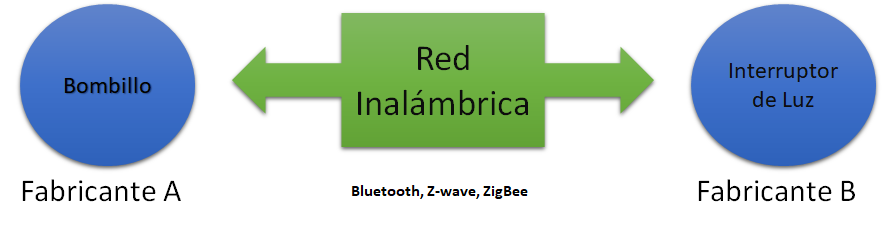
\includegraphics[scale=0.4]{./Figuras/d2d.png}
\caption{Modelo dispositivo a dispositivo}
\label{fig:d2d}
\vspace*{-10pt}
\end{figure}

  
\subsection{Comunicación Dispositivo a la Nube}
En el modelo de comunicación dispositivo a la nube, la conexión del dispositivo se conecta directamente a una nube (propia o federada) usando un proveedor de servicio (figura \ref{fig:d2n}). Este enfoque frecuentemente se aprovecha de los mecanismos de comunicación como redes celulares o la infraestructura de procesamiento de una  organización de manera directa para establecer la conexión entre el dispositivo y el servicio en la nube.
\begin{figure}[htb]
\centering
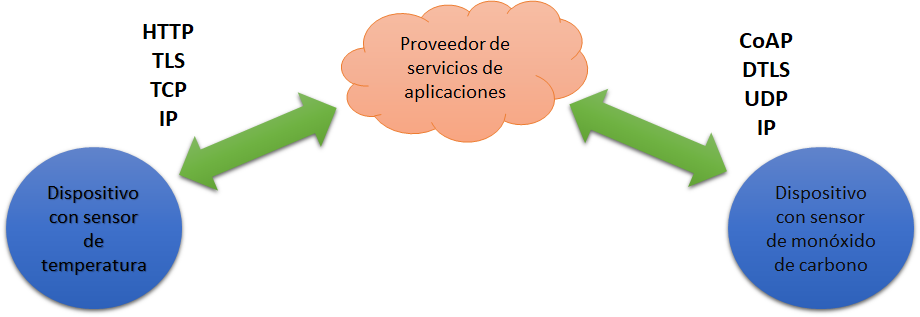
\includegraphics[scale=0.4]{./Figuras/d2n.png}
\caption{Modelo dispositivo a la nube}
\label{fig:d2n}
\vspace*{-10pt}
\end{figure}

\subsection{Comunicación Dispositivo a Puerta de Enlace}
El modelo de comunicación dispositivo a puerta de enlace establece una dispositivo o capa intermedia que concentre todas las comunicaciones (hub o broker) entre los dispositivos y de allí de ser necesario a otros fragmentos de la red o a internet (figura \ref{fig:d2g}). La ventaja de este enfoque es la capacidad de operar de manera centralizada parte de las comunicaciones de los dispositivos. Muchos protocolos están basados en el principio del paradigma de cliente-servidor por lo que este se adapta de manera natural al modelo.
\begin{figure}[htb]
\centering
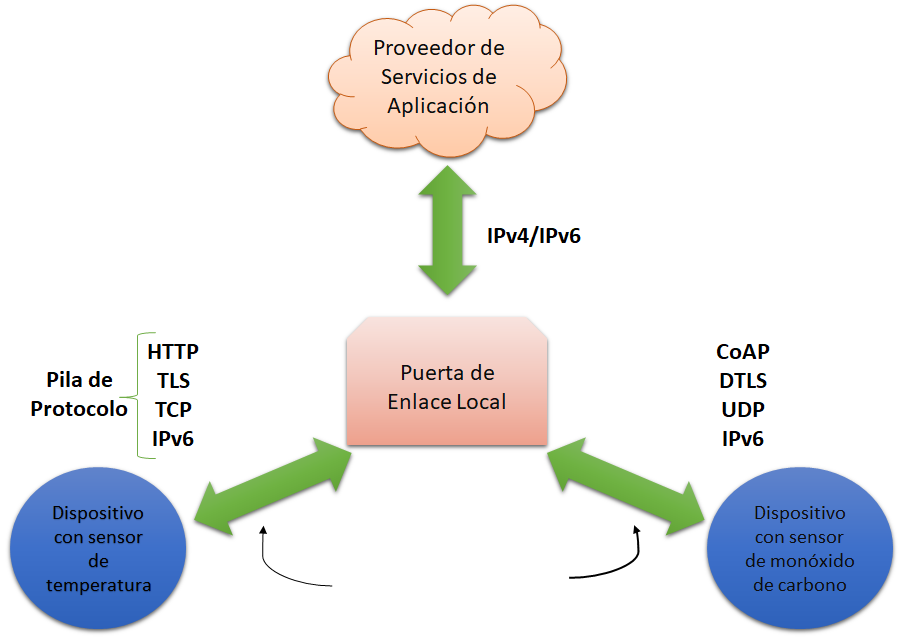
\includegraphics[scale=0.4]{./Figuras/d2g.png}
\caption{Modelo dispositivo a puerta de enlace}
\label{fig:d2g}
\vspace*{-10pt}
\end{figure}

\subsection{Comunicación Dispositivo a Intercambio de Datos en Back-end}
Este modelo es una forma automatizada de conexiones, en donde el dispositivo envía los datos a una o más APIs para de manera transparente, haciendo que este pueda intercambiar la información entre servicios que no necesariamente están estructurados o que pertenecen a un tercero (figura \ref{fig:d2b}). Particularmente este modelo es útil cuando se requiere que la información sea fácilmente accesible a través de múltiples plataformas o sistemas independientes.
\begin{figure}[htb]
\centering
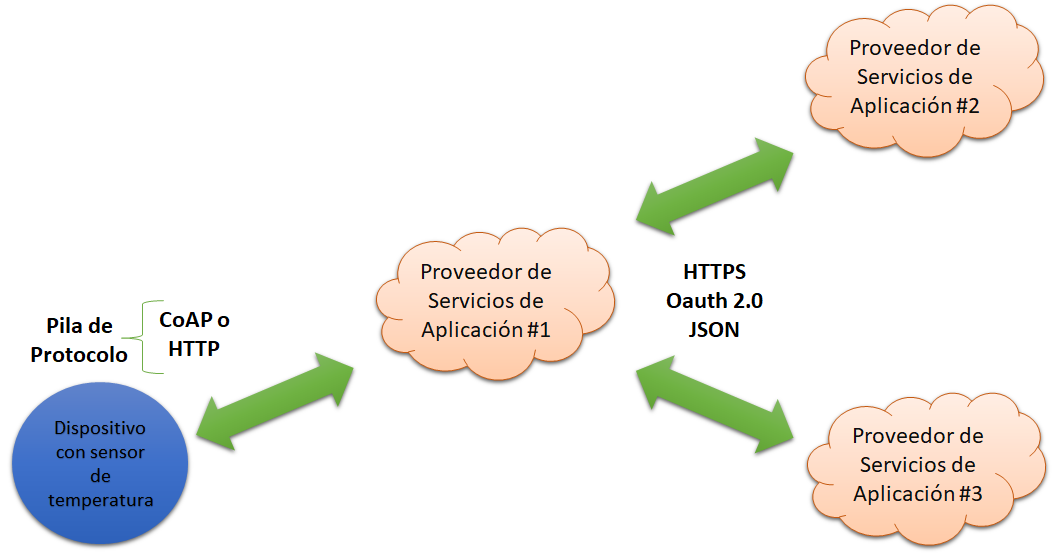
\includegraphics[scale=0.4]{./Figuras/d2b.png}
\caption{Modelo dispositivo a intercambio de datos en back-end}
\label{fig:d2b}
\vspace*{-10pt}
\end{figure}

\section{Aplicaciones del Internet de las Cosas}
Si observamos la variedad de dispositivos distintos que encontramos tanto en la vida diaria como si pensamos en términos de los sistemas altamente industrializados, se hace evidente que la cantidad de distintos nichos donde el tener sensores o elementos actuadores hace que muchos procesos se vuelvan tanto dinámicos como reactivos. Las posibilidades de adopción dispositivos interconectados en flujos para automatizar procesos es algo que se está proporcionando la base de lo que llamamos computación ubicua.

Podemos categorizar según las formas de acción y su características, varios campos donde el internet de las cosas tiene y tendrá un impacto significativo para las personas y organizaciones. En la tabla \ref{tabla:categorias_dispositivos} podemos observar alguna de esas categorías y ejemplos de tecnologías acordes.\cite{tablaiot}

\begin{table}[ht]
\centering
\begin{tabular}{| m{3.2cm}| m{4.5cm}| m{6.6cm}|}
\hline
\multicolumn{3}{|c|}{Dispositivos de Internet de las Cosas} \\
\hline 
\centering Uso & \centering Descripción & \centering Ejemplos \tabularnewline \hline
Personas & Dispositivos acareados o implantados en el cuerpo humano & Dispositivos (tecnologías vestibles o digeribles) para monitorear y mantener la salud y el bienestar. Administración de tratamientos, incremento en desempeño del ejercicio físico \\ \hline
Hogar & Casas y edificios & Control de objetos y recursos del hogar y sistemas de seguridad\\ \hline
Ventas & Tiendas y distribuidores a minoristas & Tiendas, bancos, restaurantes, estadios, cualquier lugar donde un consumidor obtenga un producto o un servicio. Ofertas en tiendas, optimización de inventarios \\ \hline
Oficinas & Espacios de trabajo y de generación de conocimiento & Administración de recursos, seguridad en las oficinas. Productividad mejorada \\ \hline
Fabricas & Entornos de producción estandarizados & Lugares donde tengan rutinas repetitivas de trabajo, incluyendo granjas o lineas de producción. Operaciones eficientes, uso de equipamiento optimizado y de inventarios \\ \hline
Lugares de Construcción y extracción de material & Producción de materias primas & Infraestructuras en Minas, Petroleo y gas. Mantenimiento predictivo; seguridad laboral \\ \hline
Vehículos & Sistemas dentro de vehículos & Vehículos incluyendo carros, camiones, barcos, aviones y trenes. Mantenimiento basado en condiciones del sistema. Diseños basados en uso. Analítica preventas \\ \hline
\end{tabular}
\caption{Dispositivos de Internet de las Cosas basados en su campo de uso según McKinsey Global Institute}
\label{tabla:categorias_dispositivos}
\end{table}

\subsection{Hogares}
En los ambientes domésticos, tecnologías como el IoT son de rápida adopción. Ya podemos observar una amplia gama de distintos dispositivos que van desde bombillos inteligentes, pasando por artefactos de linea blanca hasta elementos estructurales como sensores en tuberías que permiten tener un nivel no solo de automatización sobre labores que tradicionalmente son tediosas o difíciles de realizar.\\

Las tecnologías IoT dentro de los hogares permiten tener una amplia posibilidad de personalización y comodidad, ademas que una de las promesas es que al operar obteniendo datos ambientales y de los recursos utilizados puede ajustar y optimizar su utilización lo que representa un nivel de eficiencia que antes no era posible verificar a tan alto detalle. También es posible ahora generar una serie de tareas programadas  o rutinas diarias de los habitantes, que van desde aprovechar la luz solar en las habitaciones, limpieza de robots de las habitaciones o incluso ciertos aspectos de cuidados de mascotas también son posible ahora de administrar gracias a dispositivos inteligentes.\\

Hablando del manejo y monitoreo de recursos también ahora se abre la posibilidad de atender fenómenos recurrentes o críticos. Por ejemplo, sensores en tuberías pueden determinar si el flujo y la calidad de agua es adecuado para el consumo de la vivienda, pero también determinar si existe alguna anormalidad como filtraciones. Otro caso donde puede verse uso son los sistemas de calefacción y aire acondicionados basados en termostatos inteligentes que se adaptan a la temperaturas existentes junto con otros sensores como los de movimientos dentro de una habitación para determinar la exigencia de tener una temperatura adecuada pero teniendo en cuenta el ahorro energético.\\ 

Aspectos como la seguridad también se hacen presentes en esta categoría. Los ya tradicionales sistemas de circuitos cerrados ahora son capaces de orquestarse junto con sensores de movimiento para poder determinar un escenario de intrusión o daños a la propiedad. También mediciones como los niveles de CO2 y otros gases pueden alertar a los interesados sobre condiciones potencialmente peligrosas para los habitantes, incluso con la capacidad de alertar a las autoridades sobre el hecho anormal. 

\subsection{Industrias}
Uno de los sectores con experiencia en la adopción de dispositivos con amplia variedad de sensores y actuadores son las industrias. Desde procesos roboticos cuya tolerancia sea mínima o flujos de tareas criticas para las operaciones  se han aprovechado de esto durante años. Sin embargo la llamada industria 4.0 ahora agrega el factor de la interconexión de los sistemas con los dispositivos para presentar estados e información en tiempo real de los procesos automatizados.\\

Con la información obtenida de todos sensores implicados en los procesos automatizados los gerentes pueden entender de mejor forma se debe proceder a realizar una o mas tareas, ademas de ayudar a optimizar y encontrar puntos de mejorasen  todas las etapas del proceso de producción, desde el suministro, el desarrollo y la creación, ahorrando tiempo y dinero al mismo tiempo\cite{ibmiotindustria}.\\

La retroalimentación que se va generando en las automatizaciones debido a la existencia de estos dispositivos a manera de diagnostico ayudan a poder hacer ajustes de manera inmediata en cadenas de producción y lineas de ensamblaje. Otro aspecto positivo es tener la capacidad de monitoreo y funcionamiento optimo de maquinaria, de forma de realizar mantenimientos preventivos, lo que a la larga representa una reducción de costes y una mejora en la vida útil de las herramientas. 

\subsection{Transporte}
En el caso del transporte, tanto público como privado las oportunidades que representa la capacidad de agregar sensores de manera transversal a la infraestructura existente es uno de los focos que tanto fabricantes, reguladores y gobiernos desean alcanzar. La revolución de los automóviles  con capacidades de conducción autónoma es un ejemplo claro de como los sensores son capaces de brindar los datos necesarios para la toma de decisiones de los sistemas de control del automóvil sin asistencia y esa información recolectada es también útil para entrenar modelos de inteligencia artificial que permitan elevar el nivel de autonomía en la conducción de futuros modelos\cite{ibmiottransporte1}.\\

Otro punto que se benefician es en la cadena de suministros de repuestos. Un medio de transporte que es capaz de diagnosticar anomalías hace posible que se genere una cadena de producción directa a las necesidades requeridas, desde la fabrica de la parte hasta la solicitud de chequeo por parte del usuario.\\ 
 
En los sistemas públicos de transporte se benefician de poder traducir los datos en predicciones y en alertas para los usuarios, para ajustar itinerarios y también para poder masificar los servicios a mas personas, adapatandolo a las necesidades del entorno o del momento.\\

\subsection{Comercio y Logística}
El comercio de bienes y servicios se ajusta a los modelos de intenet de las cosas al tener una observabilidad que no se tenia previamente. Desde sensores que dan estado de un producto desde su producción hasta el momento en que es adquirido y garantizan su calidad hasta datos de localización para la vigilancia de mercancías son tecnologías que ya en la actualidad se utilizan trayendo beneficio a productores como a consumidores en general, haciendo mas transparente la cadenas de producción, buscando eficiencia  y sostenibilidad como factores importantes en la actualidad.\\

Por el lado de la logística el rastreo de bienes, el intercambio de información de inventarios de manera automática basados en la identificación de productos entre proveedores, minoristas y consumidores finales genera confianza y representa nuevo niveles de seguridad, sobre todo al momento de hacer entregas de mercancías.

\subsection{Tecnologías Vestibles}
Los weareables o tecnologías vestibles es uno de esos ámbitos en donde poco a poco se esta encontrando un nicho entre las personas. Desde relojes inteligentes, lentes para realidad aumentada y realidad virtual, prendas de vestir que vigilan nuestros signos vitales, entre otros muchos ejemplos son la forma que el internet de las cosas toma forma para esta categoría. La miniaturización de sensores y de elementos de computo está haciendo posible poder crear dichos elementos y que sean cada vez mas comunes en la vida cotidiana a pesar de retos como el consumo energético de los sensores y de las comunicaciones que estos realizan\cite{ibmappsiot}.\\

Accesorios como relojes inteligentes que son capaces de leer múltiples variables fisiológicas de forma de brindar un panorama general de la salud y otras características personales o trajes especiales, utilizados sobre todo en los deportes donde se busca tener una observación mas marcada del desempeño del deportista los dispositivos ayudan a brindar una mejor perspectiva de cara a entrenamientos y de encontrar métodos para alcanzar mas rendimiento brindando métricas en tiempo real como de forma histórica.

\subsection{Medicina y Salud}
Muy a la par de las tecnologías vestibles, el área de la salud en general se ve beneficiada de la capacidad de poder obtener lecturas de variables fisiológicas así como de los signos vitales que puedan presentar los pacientes  tanto en tiempo real como a lo largo de una intervención o de un tratamiento, así poder adaptar procedimientos, medicinas, dietas de los pacientes en búsqueda de una mas rápida evolución y mejora de las personas.\\

También podemos ver un avance en la efectividad de tratamientos médicos suministrados gracias a la capacidad de obtener la información de manera mas rápida y global por la presencia de esos sensores en los dispositivos que lleven los pacientes, sumando a la tendencia de poder brindar cada vez más tratamientos personalizados \cite{ibmiotmedicina}. Ademas la conectividad del sistema de atención de la salud a través del internet de las cosas, hace hincapié en las necesidades del paciente, es decir, tratamientos proactivos, precisión mejorada cuando se trata de diagnostico, la intervención oportuna por parte del personal de salud, en miras de una medicina cada vez mas preventiva en vez de una que sea reactiva. 

\section{Interoperatividad entre Infraestructuras y Dispositivos}
hue
\subsection{Ecosistemas}
hue
\subsection{Restricciones}
hue
\subsection{Riesgos}
hue
\subsection{Sistemas Heredados}
hue
\subsection{Configuración de dispositivos}
hue

\section{Protocolos y Estándares Utilizados}
hue
\subsection{Protocolos}
hue
\subsubsection{HTTP}
hue
\subsubsection{MQTT}
hue
\subsubsection{IPv4 e IPv6}
hue
\subsection{Estándares}
hue
\subsubsection{Bluetooth}
hue
\subsubsection{Redes Celulares}
hue
\subsubsection{NFC}
hue
\subsubsection{Wifi}
hue
\subsubsection{Zigbee}
hue
\subsubsection{Z-Wave}
hue

\section{Seguridad}
hue.
